
\section{Enumerating Gröbner fans and Code Ideals}
\label{sec:enumerate}

Now that the mathematical background is given, the specific parts which are needed to implement the software and the connection between linear codes and Gröbner bases will be presented. The first section deals with enumerating all Gröbner bases with the help of breadth-first and reverse search followed by the degree compatible Gröbner bases.
After that, linear codes will be presented and to connect these two topics together, code ideals will be defined. 

\subsection{Enumerating Gröbner fans}
\label{subsec:enumerate}

In this section, two algorithms will be explained with the  purpose to enumerate the Gröbner fan.
To compute all Gröbner bases from a toric ideal $I_A$ , it is necessary to search the \textit{edge graph} of a Gröbner fan.\\
Two reduced Gröbner bases with respect to a term order covered by the generic weight vectors $c_{1}$, $c_{2}~$ are said to be adjacent if the two Gröbner cones share a common \textit{facet}. Given a reduced Gröbner basis with respect to the weight vector $c$, \textit{facet binomials} can be defined as follows.

\begin{env_definition}[Facet Binomial]
\cite{tigers}
The binomial $x^{\upalpha_{k}}-x^{\upbeta_k} \in \mathcal{G}_c~$, $\mathcal{G}_c~$is a reduced Gröbner basis with respect to the weight vector $c$, is a facet binomial of $\mathcal{G}_c$ if and only if there exists a vector $u \in \mathbb{R}^{n}$ which satisfies :

\begin{itemize}
\item
$ \lbrace \upalpha_{i} \cdot u > \upbeta_{i} \cdot u : i = 1, \dots , t, i \neq k \rbrace  
$
\item
$ \lbrace \upbeta_{k} \cdot u > \upalpha_{k} \cdot u \rbrace .$
\end{itemize}


\end{env_definition}
Computing the facet binomials of a reduced Gröbner basis $\mathcal{G}$ can be computationally expensive, because it is needed to solve as many linear programs as the cardinality of $\mathcal{G}$. Algorithm \ref{alg:facetsLP} for finding the facets can be as follows.

\newpage

\begin{algorithm}
\caption{Finding the facets of a reduced Gröbner bases of $I_A$ \cite{tigers}}
\label{alg:facetsLP}
\label{facets}
\begin{algorithmic}[1]

\Input
Reduced Gröbner basis $ \mathcal{G} = \lbrace \underline{x}^{a_{i}} - {x}^{b_{i}} : i = 1,\dots,t  \rbrace $ of $I_A$
\Output The facet binomials of $\mathcal{G}$
\State Facets := $\emptyset$

\For{\textbf{each} binomial $\underline{x}^{a_{i}} - {x}^{b_{i}}$ in $\mathcal{G}$}
\If{${a}_{i} - {b}_{i} \notin \textrm{cone generated by } \{{a}_{j} - {b}_{j} : \underline{x}^{a_{j}} - {x}^{b_{j}} \in \mathcal{G}, i \neq k \} $}
\State Facets := Facets $~\cup~\{{x}^{a_{i}} - {x}^{b_{i}} \} $
\EndIf

\EndFor \\
\Return Facets
%\EndProcedure
\end{algorithmic}
\end{algorithm}

%TODO Kleines Beispiel mit dem Simplexalgorithmus
\begin{env_example}\normalfont

% {a-e, b^2-1, b*d-e*f, b*e-d*f, b*f-d*e, c-e, d^2-1, d*e*f-b, e^2-1, f^2-1}
Given the reduced Gröbner basis \\
 $\mathcal{G} = \{x_1 - x_5,~x_{2}^{2}-1,~x_{2}x_{4}-x_{5}x_{6},~x_{2}x_{6}-x_{4}x_{5},~x_{3}-x_{5},~x_{4}^{2}-1,~x_{4}x_{5}x_{6}-x_{2},~x_{5}^{2}-1,~x_{6}^{2}-1  \}~$ and it shall be determined if the term $x_{2}x_{4}-x_{5}x_{6}~$ is a facet or not.
 With linear programming, it must be checked if the vector $b = {\left(0,1,0,1,-1,-1\right)}^{T}$ can be expressed by the matrix multiplication $A \cdot x = b~$, where \\
 \[
 A =
 \begin{pmatrix}
 1  & 0 & 0  & 0 & 0 & 0  & 0 & 0\\ 
 0  & 2 & 1  & 0 & 0 & -1 & 0 & 0\\  
 0  & 0 & 0  & 1 & 0 & 0  & 0 & 0\\ 
 0  & 0 & -1 & 0 & 2 & 1  & 0 & 0\\
 -1 & 0 & -1 & 1 & 0 & 1  & 2 & 0\\
 0  & 0 & 1  & 0 & 0 & 1  & 0 & 2
 \end{pmatrix} 
 .\] 
  
 Now the linear program can be set up to 
 \[
 	\begin{array}{lrcl}
 	\textrm{ }   & Ax    & =    & b   \\
 	\textrm{subject to}  & x     & \geq & 0
 			    
 	\end{array}
 \]
 

\begin{flushright}
$\lozenge$
\end{flushright}
\end{env_example}
\newpage 
Another way to find the facets without linear programming is possible with the property of the following leading ideals.

Let $\mathcal{G}_{c} $ be a reduced Gröbner basis with respect to a generic weight vector $c$. Then $x^{a} - x^{b}$ is a facet binomial of $\mathcal{G}_{c}$ only if $lt_{c}(I_{a})$ (see definition \ref{def:initial}) is the initial ideal of \[W_{a - b} = \langle x^{a}-x^{b}\rangle~+~ \langle x^{c}~|~x^{c}~\textrm{is a minimal generator of~} lt_{c}(I_{a}), x^{c} \neq x^{a} \rangle \] \cite{tigers}.
With the help of this property it is possible to define an algorithm to find a superset of facet binomials of a reduced Gröbner basis.

\begin{algorithm}
\caption{Finding a superset of the facet binomials
of a reduced Gröbner basis of $I_A$ \cite{tigers}}
\label{alg:facetSS}
\begin{algorithmic}[1]

\Input
Reduced Gröbner basis $ \mathcal{G}_{c} $ of $I_A$
\Output A superset SS of the facet binomial $\mathcal{G}_{c}$
\State SS := $\emptyset$
\For{\textbf{each} $x^{a} - x^{b} \in \mathcal{G}_{c}$}
\State $W_{a - b} := \langle x^{a}-x^{b}\rangle$
$~+~ \langle x^{c} \rangle$ \Comment{$x^{c}$ is defined as before}
\If{ $lt_{c}(I_{A})~$ is the leading ideal of $W_{a-b}$ with respect to $x_{a}>_{c}x_{b}$}
\State SS := SS $\cup~ \{x^{a}-x^{b} \}$

\EndIf
\EndFor \\
\Return SS

%\EndProcedure
\end{algorithmic}
\end{algorithm}
 

In the example \ref{ex:groebnerfan} the facet binomials of a Gröbner cone determine the border to an other Gröber cone.
In order to traverse from a Gröber base $\mathcal{G}_c$ to a neighboured Gröbner base $\mathcal{G}_{c'}$ with the certain facet $x^{\upalpha}-x^{\upbeta} $, a procedure making a local change from $\mathcal{G}_c$ to $\mathcal{G}_{c'}$ is required.
This procedure is called flip and is presented in algorithm \ref{alg:flip}. 
\newpage


\begin{algorithm}
\caption{Local change of reduced Gröbner bases in $I_A$ \cite{tigers}}
\label{alg:flip}
\begin{algorithmic}[1]

\Input
Reduced Gröbner basis $ \mathcal{G} $ of $I_A$

    A prescribed facet binomial $ \underline{x}^{a}_{i} - x^{b}_{i} \in \mathcal{G} $
%\Comment {The weight vector inducing $\mathcal{G}$ is generic and the leading terms are underlined}
\Output The reduced Gröbner basis is adjacent to $\mathcal{G}$ in which $ \underline{x}^{b}_{i} - x^{a}_{i} $ is a facet binomial.
\State Old 
$:= \lbrace \underline{x}^{a}_{i} - x^{b}_{i} \rbrace \cup
 \lbrace \underline{x}^{a}_{j} : \underline{x}^{a}_{j} - x^{b}_{j} \in \mathcal{G},
 j \neq i \rbrace $ \Comment{Prescribed Facet and leading terms only in Old }
 \State Temp $:= \lbrace \underline{x}^{b}_{i} - x^{a}_{i} \rbrace \cup 
 \lbrace \underline{x}^{a}_{j} : x^{a}_{j} \in Old  \rbrace $
 \Comment{Flipping the facet Binomial}
 \State New := Reduced Gröbner basis with respect to the new marking 
 \Comment{See algorithm \ref{alg:buchberger}.}
 \State $\mathcal{G}' = \left\lbrace \underline{x}^{b}_{i} - x^{a}_{i} \right\rbrace  $
 
 \For{\textbf{each} monomial h in New}
 \State Reduce $h$ with $\mathcal{G}$ to obtain the monomial $h'$.
 \State Add $h-h'$ to $\mathcal{G}'$ with $h$ marked as the leading term.
 \EndFor
 \State Auto-reduce $\mathcal{G}'$ to get $\mathcal{G}_{new}$
 \Comment{no term shall be divisible by a leading term}

%\EndProcedure
\end{algorithmic}
\end{algorithm}

This algorithm is correct and can terminate \cite{tigers}.
The main advantage of the algorithm is that no weight vectors must be stored or computed.
Weight vectors are carried implicitly and that is possible due to the binomial structure that this subroutine generates for every Gröbner basis. For this work \\ flip$({x}^{a}_{i} - x^{b}_{i},~\mathcal{G})$ means that algorithm \ref{alg:flip} is applied with the needed input.

\begin{env_example}\normalfont
Consider the reduced Gröbner basis with respect to a term order $\succ~$: $\mathcal{G}= \{x_{6}^{2}-1,~x_{5}^{2}-1,~x_{4}x_{5}x_{6} -x_{2},~x_{4}^{2}-1,~x_{3}-x_{5},~x_{2}x_{6}-x_{4}x_{5},~x_{2}x_{5}-x_{4}x_{6},~x_{2}x_{4}-x_{5}x_{6},~x_{2}^{2}-1,~x_{1}-x_{5}  \} $.

Applying the procedure flip$(x_{3}-x_{5}, \mathcal{G}$) leads to:

Old := $\{x_{3}-x_{5},~x_{6}^{2},~x_{5}^{2},~x_{4}x_{5}x_{6} ,~x_{4}^{2},~x_{2}x_{6},~x_{2}x_{5},~x_{2}x_{4},~x_{2}^{2},~x_{1} \} $ \\
Temp := $\{x_{5}-x_{3},~x_{6}^{2},~x_{5}^{2},~x_{4}x_{5}x_{6} ,~x_{4}^{2},~x_{2}x_{6},~x_{2}x_{5},~x_{2}x_{4},~x_{2}^{2},~x_{1} \} $

Now the new Gröbner basis has to be calculated, but first it useful to know that all pairs of binomials which have the least common multiple 1 will be auto-reduced to zero. In other words, it is only necessary to form the S-Pairs of binomials that are not relatively prime.

\begin{align*}
	S(x_{5}-x_{3},x_{5}^{2}) &= x_{3}x_{5} \\
	S(x_{5}-x_{3},x_{4}x_{5}x_{6}) &= x_{3}x_{4}x_{5} \\
	S(x_{5}-x_{3},x_{2}x_{5}) &= x_{2}x_{3} \\
	S(x_{5}-x_{3},x_{3}x_{5}) &= x_{3}^{2}
\end{align*}

Now the new Gröbner basis $\mathcal{G}'$ shall be filled with all monomials from $\mathcal{G}$.
The underlined terms are the terms reduced with $\mathcal{G}~$ and will be the new non-leading terms.
\begin{align*}
	x_{3}x_{5} &= x_{5}(x_{3}-x_{5}) + 1(x_{5}^{2}-1) &+ \underline{1} \\
	x_{3}x_{4}x_{6} &= x_{4}x_{6}(x_{3}-x_{5}) + 1(x_{4}x_{5}x_{6}-x_{2}) &+ \underline{x_{2}} \\
	x_{2}x_{3} &= x_{2}(x_{3}-x_{5}) + 1(x_{2}x_{5}- x_{4}x_{6}) &+ \underline{x_{4}x_{6}} \\
	x_{3}^{2} &= x_{3}(x_{3}-x_{5}) + x_{5}(x_{3}x_{5}) + 1(x_{5}^{2}-1)&+\underline{1} \\
	x_{1} &= (x_{1}-x_{5}) + (x_{5}-x_{3}) &+\underline{ x_{3}} \\
	x_{2}x_{6} &= (x_{2}x_{6}-x_{4}x_{5}) + x_{4}(x_{5}-x_{3}) &+\underline{ x_{3}x_{4}} \\
	x_{2}x_{4} &= (x_{2}x_{4}-x_{5}x_{6})+ x_{6}(x_{5}-x_{3}) &+\underline{x_{3}x_{6}}
\end{align*}

The other monomials of $\mathcal{G}~$ are not notated here because they did not get a new non-leading term.

This results to the Gröbner base : \\
$\mathcal{G}' = \{x_{5}-x_{3},~x_{6}^{2}-1,~x_{5}^{2}-1,~x_{4}x_{5}x_{6}-x_{2},~x_{4}^{2}-1,~ x_{2}x_{6}-x_{3}x_{4},~x_{2}x_{5}-x_{4}x_{6},~x_{2}x_{4}-x_{3}x_{6} ,~x_{2}^{2}-1,x_{1}-x_{3},~x_{3}x_{5}-1,~x_{3}x_{4}x_{6}-x_{2},~x_{2}x_{3}-x_{4}x_{6},~x_{3}^{2}-1 \}.$ \\
This Gröbner base is not reduced yet. After cancelling all binomials whose terms are divisible by some other leading terms the new reduced Gröbner basis is 
$\mathcal{G}_{new} = \{x_{5}-x_{3},~x_{6}^{2}-1,~x_{4}^{2}-1,~x_{2}x_{6}-x_{3}x_{4},~x_{2}x_{4}-x_{3}x_{6},~x_{2}^{2}-1,~x_{1}-x_{3},~x_{3}x_{4}x_{6}-x_{2},~x_{2}x_{3}-x_{4}x_{6},~x_{3}^{2}-1 \}.$

\begin{flushright}
$\lozenge$
\end{flushright}
\end{env_example}


\subsubsection{Breadth first search}

In this section an algorithm to enumerate the edge graph of a Gröbner fan via breath-first search and its drawbacks are presented.

\begin{algorithm}
\caption{Enumerating the edge graph of the Gröbner fan via breath-first search \cite{tigers}}
\label{alg:breath}
\begin{algorithmic}[1]

\Input
Any reduced Gröbner basis $ \mathcal{G}_0 $ of $I_A$
\Output All reduced Gröbner bases of $I_A$, (all vertices of the edge graph)
\State Todo := $\left[ \mathcal{G}_0 \right]  $
\State Verts := $\left[ \right] $
\While{Todo $\neq \emptyset$ }
\State $\mathcal{G}$ := first element in (Todo)
\State Remove $\mathcal{G} $ from Todo
\State add $\mathcal{G}$ to Verts 
\State determine list L of facet binomials of $\mathcal{G} $
\Comment{With linear programming}
 \For{\textbf{each} $x^{\upalpha}-x^{\upbeta} \in ~$ L  }
 \State $\mathcal{G}' =~$ flip($\mathcal{G},x^{\upalpha} - x^{\upbeta} $)
 \If{$\mathcal{G}' \notin \mathrm{Todo} \cup \mathrm{Verts}  $}
 \State add $\mathcal{G}'$ to Todo
 \EndIf
 \EndFor
\EndWhile 
\Return Verts

%\EndProcedure
\end{algorithmic}
\end{algorithm}

This algorithm is intuitive but has the drawback that every vertex of the edge graph must be stored and every vertex must be checked against all other vertices if it is a new vertex or not. 
The more vertices the edge graph has, the more expensive the calculation will be. Also the need of memory will arise if a Gröbner fan has a lot of cones.
 
 \newpage

\subsubsection{Reverse search tree}
The disadvantages can be canceled out with a memoryless algorithm, which runs linear depending on the size of output. The idea is to enumerate the edge graph with depth-first reverse search. The result will be a directed subgraph of the edge graph, called reverse search tree $T_{\succ}(I_{A}) $.\\
\begin{env_definition}[Mismarked Polynomial]
\cite{tigers}
A polynomial $f$ that has been marked with respect to the monomial order $>$  is mismarked with respect to the monomial order $>'$  .
\end{env_definition}

\begin{env_example}\normalfont
Consider the reduced Gröbner base \\ $\mathcal{G} = \left\lbrace x^{2}y-z,y^{2}-xz, zy-xy^{2}z \right\rbrace $ 
with a certain monomial order $>$, which is not the lexicograpic order.
Then, the second and last term are clearly mismarked with respect to $>_{lex}$.

Applying the flip-procedure $(\mathcal{G},y^{2}-xz)$ leads to the Gröbner base \\ $\mathcal{G} = \{x^{2}y-z,xz^{2}-y^{2}, zy-xy^{2}z \} $. Now only the last binomial is mismarked and using flip($\mathcal{G}$, $zy-xy^{2}z$) the result is the reduced Gröbner basis with respect to the lexicographic order $\mathcal{G} = \{xy^{2}z -xy,~xz^{2}-y^{2},~xy-z \} $. Note that every monomial can not be divided by the leading terms, so all Gröbner bases are reduced and no auto-reduce is necessary.
 
\begin{flushright}
$\lozenge$
\end{flushright} 
\end{env_example}


The \textit{reverse search tree} $T_{\succ}(I_{A}) $ with a given monomal order $ > $ can be defined as follows:
\begin{env_definition}[Reverse Search Tree]
\label{def:reverse}
\cite{tigers} For two reduced Gröbner bases $\mathcal{G}_{i}$ and $\mathcal{G}_{j}~$, $[\mathcal{G}_{i},\mathcal{G}_{j} ]~$ directed from $\mathcal{G}_{i}~$to $\mathcal{G}_{j}~$ is an edge of $~T_{\succ}(I_{A}) $ if $\mathcal{G}_{i}$ is obtained from $\mathcal{G}_{j}$ by the algorithm \ref{alg:flip} flip$(x^{\upalpha} - x^{\upbeta},~\mathcal{G}_{i}).$ $x^{\upalpha}$ is lexicographically maximal among all facet binomials of $\mathcal{G}_{i}$, that are mismarked with respect to $>$.
\end{env_definition}


\newpage

It can be shown that the reverse search tree is an acyclic graph with a unique sink and from any reduced Gröbner basis of $\mathcal{G}_{c} $ of a toric ideal $I_{A}$, there is a unique path to the sink $\mathcal{G}_{>}$ \cite{tigers} .
Unlike the Gröbner walk procedure, there are still no weight vectors involved, but in return every facet of the Gröebner cone must be computed, which can be computionally expensive for reduced Gröbner basis with many polynomials.

\begin{algorithm}
\caption{Enumerating the edge graph of the Gröbner fan via reverse search \cite{tigers}}
\label{alg:reverse}
\begin{algorithmic}[1]

\Input
Any reduced Gröbner basis $ \mathcal{R}_{>} $ of $I_A$ and its term order $>$
\Output All reduced Gröbner bases of $I_A$, (all vertices of the edge graph)
\State $\mathcal{G} := \mathcal{R}_{>}$;$~j := 0$;$~L := $ list of facet binomials of $\mathcal{G}$ marked by $>$
\State add $\mathcal{G}$ to output
\Repeat
\While{ $ j < \left|L\right| $ }

\State j := j + 1
\State $\mathcal{G}':= $ flip($\mathcal{G}$,$L[j]$);

\If{ $[\mathcal{G}',\mathcal{G}] \in T_{>}(I_{A}) $ }
\Comment{ Check for adjacency }
\State $\mathcal{G} := \mathcal{G}' $;   $~j := 0$
\State $ L := $ list of facet of $\mathcal{G}$ marked by $>$
\State add $ \mathcal{G}$ to output

\EndIf 

\EndWhile

\If{$ \mathcal{G} \neq \mathcal{R}_{>}$}
\State $\mathcal{G}' :=~$ unique element such that $[\mathcal{G}',\mathcal{G}] \in T_{>}(I_{A}) $
\State $j := 0$
\State $L := $ list of facets of $\mathcal{G}'$ marked by $>$

\Repeat
\State $j := j + 1$
\Until{the common facet of $\mathcal{G}$ and $\mathcal{G}'$ is the $j$-th facet of $L$ }

\EndIf

\Until{$\mathcal{G} = \mathcal{R}_{>}$ and $ j = \left|L\right| $ }


%\EndProcedure
\end{algorithmic}
\end{algorithm}

\newpage

\begin{env_example}\normalfont
Consider the ideal with the reduced Gröbner basis with respect to the lexicographic order $x_{1} > \ldots > x_{6} $
\[ \mathcal{G} = \{x_{1} - x_{2}, x_{3} - x_{4}, x_{5}-x_{6} , x_{2}^{2} -1 , x_{4}^{2} - 1, x_{6}^{2} - 1 \}. \]

Applying the breath-first search algorithm for this reduced Gröbner basis results to the following edge graph.\\
Using the reverse search method, this search tree on figure \ref{fig:reverse} results.


\begin{figure}[h]
    \centering
    \begin{subfigure}[b]{0.48\linewidth}        %% or \columnwidth
        \centering
        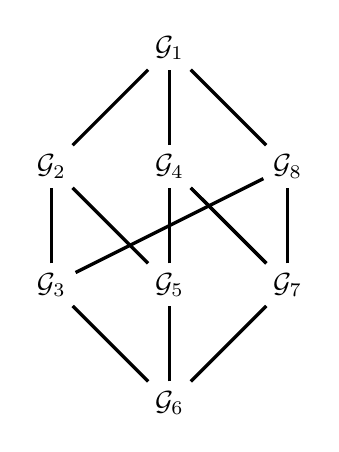
\begin{tikzpicture}[scale = 0.5]
\node (A) at (0,0) {$\mathcal{G}_{1}$};

\node (C) at (-3,-3) {$\mathcal{G}_{2}$};
\node (D) at (0,-3) {$\mathcal{G}_{4}$};
\node (B) at (3,-3) {$\mathcal{G}_{8}$};

\node (E) at (3,-6) {$\mathcal{G}_{7}$};
\node (F) at (-3,-6) {$\mathcal{G}_{3}$};
\node (G) at (0,-6) {$\mathcal{G}_{5}$};

\node (H) at (0,-9) {$\mathcal{G}_{6}$};


\draw[-, very thick] (D) to (A);
\draw[-, very thick] (C) to (A);
\draw[-, very thick] (B) to (A);

\draw[-, very thick] (E) to (D);
\draw[-, very thick] (F) to (C);
\draw[-, very thick] (G) to (D);
\draw[-, very thick] (G) to (C);
\draw[-, very thick] (E) to (D);
\draw[-, very thick] (F) to (B);
\draw[-, very thick] (E) to (B);

\draw[-, very thick] (H) to (G);
\draw[-, very thick] (H) to (F);
\draw[-, very thick] (H) to (E);
%\draw[-, very thick] (F) to (G);

\end{tikzpicture}
        \caption{Complete edge graph}
        \label{fig:breadth}
    \end{subfigure}
    \begin{subfigure}[b]{0.48\linewidth}        %% or \columnwidth
        \centering
        
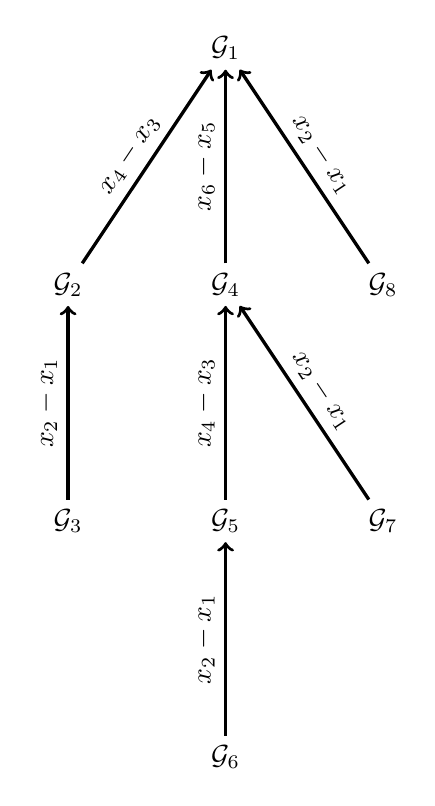
\begin{tikzpicture}

\node (A) at (0,0) {$\mathcal{G}_{1}$};

\node (C) at (-2,-3) {$\mathcal{G}_{2}$};
\node (D) at (0,-3) {$\mathcal{G}_{4}$};
\node (B) at (2,-3) {$\mathcal{G}_{8}$};

\node (E) at (2,-6) {$\mathcal{G}_{7}$};
\node (F) at (-2,-6) {$\mathcal{G}_{3}$};
\node (G) at (0,-6) {$\mathcal{G}_{5}$};

\node (H) at (0,-9) {$\mathcal{G}_{6}$};


\draw[->, very thick] (D) to node[midway, above, sloped]  {$x_{6}-x_{5}$}(A);
\draw[->, very thick] (C) to node[midway, above, sloped]   {$x_{4}-x_{3}$} (A);
\draw[->, very thick] (B) to node[midway, above, sloped]   {$x_{2}-x_{1}$} (A);

\draw[->, very thick] (E) to node[midway, above, sloped]   {$x_{2}-x_{1}$} (D);
\draw[->, very thick] (F) to node[midway, above, sloped]   {$x_{2}-x_{1}$}(C);
\draw[->, very thick] (G) to node[midway, above, sloped]   {$x_{4}-x_{3}$}(D);

\draw[->, very thick] (H) to node[midway, above, sloped]   {$x_{2}-x_{1}$}(G);


\end{tikzpicture}

        \caption{Reverse search tree}
        \label{fig:reverse}
    \end{subfigure}
    \caption{Comparison between the breath-first search and the reverse search}
    \label{fig:graph}
\end{figure}
\newpage
%thx to http://www.math.tugraz.at/~huss/new/teaching/computermathematik09/dateien/tikz_demonstration.pdf
The flipping binomials at figure \ref{fig:reverse} are written on the edges.

The Gröbner bases are:
\begin{center}
$\mathcal{G}_{1} = \{x_{1}-x_{2},x_{3}-x_{4},x_{5}-x_{6},x_{2}^{2}-1,x_{4}^{2}-1,x_{6}^{2}-1 \} $ \\
$\mathcal{G}_{2} = \{x_{1}-x_{2},x_{4}-x_{3},x_{5}-x_{6},x_{2}^{2}-1,x_{3}^{2}-1,x_{6}^{2}-1 \} $ \\
$\mathcal{G}_{3} = \{x_{2}-x_{1},x_{4}-x_{3},x_{5}-x_{6},x_{1}^{2}-1,x_{3}^{2}-1,x_{6}^{2}-1 \} $ \\
$\mathcal{G}_{4} = \{x_{1}-x_{2},x_{3}-x_{4},x_{6}-x_{5},x_{2}^{2}-1,x_{4}^{2}-1,x_{5}^{2}-1 \} $ \\
$\mathcal{G}_{5} = \{x_{1}-x_{2},x_{4}-x_{3},x_{6}-x_{5},x_{2}^{2}-1,x_{3}^{2}-1,x_{5}^{2}-1 \} $ \\
$\mathcal{G}_{6} = \{x_{2}-x_{1},x_{4}-x_{3},x_{6}-x_{5},x_{1}^{2}-1,x_{3}^{2}-1,x_{5}^{2}-1 \} $ \\
$\mathcal{G}_{7} = \{x_{2}-x_{1},x_{3}-x_{4},x_{6}-x_{5},x_{1}^{2}-1,x_{4}^{2}-1,x_{5}^{2}-1 \} $ \\
$\mathcal{G}_{8} = \{x_{2}-x_{1},x_{3}-x_{4},x_{5}-x_{6},x_{1}^{2}-1,x_{4}^{2}-1,x_{6}^{2}-1 \} $ \\
\end{center}

A lot of edges were saved which results to less computation.
\begin{flushright}
$\lozenge$
\end{flushright}
\end{env_example}




\subsection{Degree compatible Gröbner basis}
\label{subsec:degreecomp}
Computing the whole Gröbner fan can be very expensive and not every Gröbner basis is interesting.
In this section, the degree compatible Gröbner fan is introduced and how the algorithm can
be changed so that only the degree compatible Gröbner fan will be computed.\\
\begin{env_definition}[Degree compatible Gröbner basis]
\cite{dueckpaper}
A reduced \\ Gröbner basis for an ideal I with respect to a certain monomial order is
degree compatible if and only if the corresponding Gröbner cone contains the all-one vector \textbf{1}.
\end{env_definition}
Equivalent to this, the leading term of every polynomial must have the highest degree.
Since a Gröbner fan is homogeneous at $\mathbb{R}^{n}_{+}$, there will be at least one degree compatible Gröbner basis.
That is a special case can be easily determined as follows.

\begin{env_definition}[Only degree compatible Gröbner basis]
\cite{dueckpaper}
A Gröbner basis $\mathcal{G}$ with respect to a degree compatible monomial ordering $>$  is the only degree compatible Gröbner basis for an ideal if and only if
\[ deg(x^{a}) > deg(x^{b})~~ \forall~~ x^{a}-x^{b}\in \mathcal{G}. \] 
\end{env_definition}

This can be also described by the all-one vector that lies completely in a Gröbner cone of a Gröbner basis $\mathcal{G}$.
It follows that the all-one vector does not intersect with any facets if there is only one degree compatible Gröbner basis. \\

The algorithms \ref{alg:breath} and \ref{alg:reverse} can be adapted in order to compute only the degree compatible Gröbner fan.\\ 
The breadth-first search now needs a degree compatible Gröbner basis as an input. This can be achieved by applying the Buchberger Algorithm with a degree compatible monomial, for example the \textit{grlex} order. After that it is required that the Gröbner basis is checked if its is the only degree compatible basis. %see only degree compatible Gröbner basis
Also the only facet binomials $x^{a} - x^{b}$ which are allowed to be "flipped" are the binomials that satisfy the condition
deg(x$^{a}$) = deg(x$^{b}$). \\ \\
The reverse search tree can be deployed as in definition \ref{def:reverse} but with the restriction that deg(x$^{a}$) = deg(x$^{b}$) must be satisfied to traverse the degree compatible Gröbner fan.
It can be ensured by \cite{dueckpaper} that at least one such facet binomial will be found. 
The sink of the reverse search tree contains binomials that are not mismarked with respect to some degree compatible monomial order. 

   

\newpage

\subsection{Linear Codes over Prime Fields}
\label{subsec:linearcodes}
This work is focused on computing the Gröbner fan of linear codes. Now the mathematic background of the Gröbner fans is given, the linear Codes and code ideals have to be defined to give a connection between these two topics.\\ 
Let $\mathbb{F}$ be a finite field and let $n~$and $k\in \mathbb{N}~$ with $n\geq k$.
\begin{env_definition}[Linear Code]
\cite{dueckjournal} A linear code of length n and dimension k over $\mathbb{F}~$is the image $\mathcal{C}~$of a injective linear mapping $\phi~:~\mathbb{F}^{k} \rightarrow \mathbb{F}^{n}.$
\end{env_definition} 
Such a code will be denoted as an [$n,k$] code and its elements are called codewords. The codewords are written 
as row vectors. The Code $\mathcal{C}~$can alternatively be described as a row space matrix of $G \in \mathbb{F}^{k \times n}$. The rows of $G$ form a basis of $\mathcal{C}$.
The matrix $G$ is also called \textit{generator matrix} for $\mathcal{C}$.
\begin{env_definition}[Standard form]
\cite{dueckjournal}
A $[n,k]~$ code $\mathcal{C}~$is in standard form if it has a generator matrix like $G = (I_{k}| M)$, where $I_{k}$ is the $k \times k$ matrix.
\end{env_definition}


\begin{env_example}\normalfont
Consider the binary $[7,4]$ Hamming Code with its generator matrix

\[
G =
\begin{pmatrix}
1 & 0 & 0 & 0 & 1 & 1 & 0 \\ 
0 & 1 & 0 & 0 & 1 & 0 & 1 \\  
0 & 0 & 1 & 0 & 1 & 1 & 1 \\ 
0 & 0 & 0 & 1 & 0 & 1 & 1
\end{pmatrix} 
.\]

The codeword $c~$of the word $x~$is obtained with the vector-multiplication
\[
     xG = c. \\
 \]
 Let $x$ be $\left(1,0,1,0\right)$, then the codeword c results to:
 \[
      \left(1,0,1,0\right) \cdot \begin{pmatrix}
      1 & 0 & 0 & 0 & 1 & 1 & 0 \\ 
      0 & 1 & 0 & 0 & 1 & 0 & 1 \\  
      0 & 0 & 1 & 0 & 1 & 1 & 1 \\ 
      0 & 0 & 0 & 1 & 0 & 1 & 1
      \end{pmatrix}   = \left(1,0,1,0,0,0,1\right) \\
  \]
\begin{flushright}
$\lozenge$
\end{flushright} 

\end{env_example}

Two codes are equivalent if one generator matrix can be obtained from the other by permuting columns and rows.
It follows that every linear code is equivalent to a linear code in standard form \cite{dueckjournal}. \\

A linear Code $\mathcal{C}$ can be \textit{punctured} by deleting individual code symbols.
This reduces the length of the code and rises the data rate for a transmission of a code.


\subsection{Code Ideals}
\label{subsec:codeideals}
In this section, the linear codes and the Gröbner bases come together.\\
Each linear code $\mathcal{C}~$ can be associated to a binomial ideal \cite{dueckpaper}. Let $\mathcal{C}~$ be a $[n,k]$ code and let 
$\mathbb{K}[\textbf{x}]=\mathbb{K}[x_{1},\dots,x_{n}]$.
Then the \textit{code ideal} can be defined as follows:

\begin{env_definition}[Code Ideal]
\cite{dueckpaper} A code ideal $I(\mathcal{C})$ is the union between the toric ideal and a nonprime ideal $I_{p}$, such that
\begin{align*}
 I_{\mathcal{C}} & = \langle \textbf{x}^{c} - \textbf{x}^{c'} | c - c' \in \mathcal{C}  \rangle + I_{p},\\
\textrm{where} ~ I_{p} & = \langle x_{i}^{p} - 1 | 1 \leq i \leq n \rangle .
\end{align*}
\end{env_definition}

\newpage

\begin{env_example} \normalfont
 Let $\mathcal{C}_{1}~$ be a binary $[6,3]$ code with generator matrix
\[
G_{1} =
\begin{pmatrix}
1 & 0 & 0 & 0 & 1 & 0 \\ 
0 & 1 & 0 & 1 & 1 & 1 \\  
0 & 0 & 1 & 0 & 1 & 0  
\end{pmatrix} 
.\]

The associated code ideal $I(\mathcal{C})$ leads to: \newline
\begin{align*}
I(\mathcal{C}) = &\{x_{1}-x_{5},~x_{2}-x_{4}x_{5}x_{6},~x_{3}-x_{5}  \} ~\cup \\ &\{x_{1}^{2}-1,~x_{2}^{2}-1,~x_{3}^{2}-1,~x_{4}^{2}-1,~x_{5}^{2}-1,~x_{6}^{2}-1\}
\end{align*}
Note that the terms $x_{1}^{2}-1,~x_{2}^{2}-1,~x_{3}^{2}-1 $ are divisible by the leading terms of the toric ideal.
The reduced Gröbner basis $\mathcal{G}_{>}$ with respect to the lexicographic ordering $>$ with $x_{1} > \cdots > x_{6}$ is:
\begin{center}
$ \mathcal{G}_{>} = \{x_{1}-x_{5},~x_{2}-x_{4}x_{5}x_{6},~x_{3}-x_{5}  \} \cup \{x_{4}^{2}-1,~x_{5}^{2}-1,~x_{6}^{2}-1  \}  $
\end{center}

Puncturing the fourth symbol $x_4$ results to new reduced Gröbner base 
\begin{center}
$ \mathcal{G}_{>} = \{x_{1}-x_{5},~x_{2}-x_{5}x_{6},~x_{3}-x_{5}  \} \cup \{x_{5}^{2}-1,~x_{6}^{2}-1  \}  $.
\end{center}
Note that the term $x_{4}^{2}-1~$was auto-reduced.


\begin{flushright}
$\lozenge$
\end{flushright} 

\end{env_example}

 

\newpage